\section{Testing, Analysis and Evaluation}
    This chapter talks about various specifics of testing and obtained results. Test cases are presented here and references are given to originally specified requirements. Afterwards, analysis is performed on results generated by running the developed software. At the end, the last section gives a quick review of project objectives and aims.
    
    \subsection{Software Testing}
        Firstly, \cref{dataeval} discusses brief test cases that ensure that data sets are obtained properly and unzipped into required folder.
        
        Secondly, \cref{twittereval} shows what methods were used to evaluate whether twitter mining requirements are met.
        
        \cref{lstmeval} talks about how \gls{lstm} performance is evaluated, including both code listings and images showcasing overall results.
        
        Then, \cref{grapheval} describes tests that evaluate the functionality of constructing graphs, while \cref{afeval} deals with making sure that analysis and computation of \gls{af}s works as intended.
        
        Afterwards, \cref{analysis} performs an analysis on the results obtained from running the software.
        
        Lastly, \cref{softachieve} puts things into perspective showcasing how the developed software project correlates with a portion of project's objectives laid out in the introduction section.
    
        \subsubsection{Evaluation of Dataset Manager Functions} \label{dataeval}
            There are only 3 main requirements for the data set manager (see \cref{table:func1spec}). What each of the test cases do is check whether the files are in the required folder and if they are not, they are downloaded. The condition is true when the zip file is present in the folder.
            
            To make sure data is being extracted, additional check is performed to ensure that the extracted file name with file type extension exists alongside the zip file in the folder. This ensures that the data set is ready to be processed by the software (see \cref{fig:testres1}).
            
            \begin{figure}[!htbp]
                \centering
                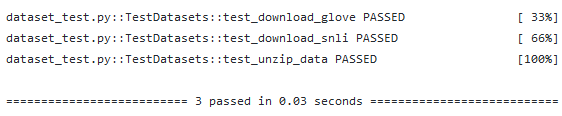
\includegraphics[scale=0.9]{img/dataset_test.png}
                \caption{Test Results for Function 1 Requirements}
                \label{fig:testres1}
            \end{figure}
        
        \subsubsection{Twitter Data Mining Evaluation} \label{twittereval}
            To evaluate the performance of Twitter miner functionality, test cases were used again. This time there are more requirements than in previous subsection, so naturally more test cases are required as well.
            
            The requirements 2.1, 2.2 and 2.7 (see \cref{table:func2spec}) involved connecting to Twitter \gls{api} and fetch new data each time the test is run. For 2.3 - 2.6, a more simple test cases were developed as those requirements deal purely with string manipulation and processing. Overall result is that all cases have passed and requirements are met as expected. \cref{fig:testres2} shows this, as each function name corresponds to a requirement listed in \cref{table:func2spec}.
            
            \begin{figure}[!htbp]
                \centering
                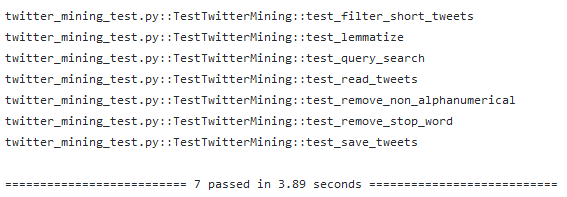
\includegraphics[]{img/twitter_mining_test.png}
                \caption{Test Results for Function 2 Requirements}
                \label{fig:testres2}
            \end{figure}
            
        \subsubsection{LSTM Performance Evaluation} \label{lstmeval}
            The main parameters for evaluating \gls{lstm} performance is accuracy and loss. Accuracy is a percentage value that shows how many samples the model predicted correctly compared to how many there are total. Loss, on the other hand, is not a percentage. It is a summation of the errors made for each example in training, validation and testing sets.
            
            \begin{lstlisting}[language=Python, caption=Accuracy Calculation, label=code:accuracy]
with tf.variable_scope('Accuracy'):
    predicts = tf.cast(tf.argmax(self.__classification_scores, 1), 
                      'int32')
    y_label = tf.cast(tf.argmax(self.__labels, 1), 'int32')
    corrects = tf.equal(predicts, y_label)
    num_corrects = tf.reduce_sum(tf.cast(corrects, tf.float32))
    self.__accuracy = tf.reduce_mean(tf.cast(corrects, tf.float32))
            \end{lstlisting}
            
            The code for evaluating accuracy is presented above (see \cref{code:accuracy}).
            
            \begin{lstlisting}[language=Python, caption=Loss Calculation, label=code:loss]
with tf.variable_scope("loss"):
    cross_entropy = tf.nn.softmax_cross_entropy_with_logits_v2(
          logits=self.__classification_scores, labels=self.__labels)
    self.__loss = tf.reduce_mean(cross_entropy)
    self.__total_loss = self.__loss + self.__weight_decay * 
          tf.add_n(tf.get_collection(tf.GraphKeys.REGULARIZATION_LOSSES))
            \end{lstlisting}
            
            Both Loss and Accuracy calculations involve dynamic variables that are adjusted as needed while the model learns and tries to maximise accuracy and reduce losses. After set amount of steps, the system prints on screen current accuracy and loss values, showing in which direction it is adapting, and whether the values are satisfactory at any given step (see \cref{code:print1}).
            
            \begin{lstlisting}[language=Python, caption=Accuracy and Loss Reporting, label=code:print1]
acc = self.__sess.run(self.__accuracy, feed_dict={self.__hyp: hyps,
                                                self.__evi: evis,
                                                self.__labels: labels,
                                                self.__input_keep: 0.1})
tmp_loss = self.__sess.run(self.__loss, feed_dict={self.__hyp: hyps,
                                                self.__evi: evis,
                                                self.__labels: labels,
                                                self.__input_keep: 0.1})
            \end{lstlisting}
            
            This process is performed during training, validation and testing cycles. Additionally, at the end of each stage (e.g. training), the overall average accuracy and loss values are calculated and printed to the user (code is not shown here in \cref{code:print1}).
            
            If the model results are satisfactory, the model is saved for future use as per software implementation details in previous chapter.
            
            Moving on to requirements, only 3.5 (see \cref{table:func3spec}) was tested using Python unit tests. This is because other requirements (3.1 - 3.4 and 3.6 - 3.8) are hard to test without investing a lot of hardware resources. Figure below shows the results of 3.5 requirement's test:
            
            \begin{figure}[!htbp]
                \centering
                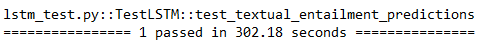
\includegraphics[]{img/test_lstm_entailment.png}
                \caption{Test Results for 3.5 Requirement}
                \label{fig:testres3}
            \end{figure}
            \FloatBarrier
            
            The long execution time is the effect of having to setup the \gls{lstm} from saved model and to run it.
            
            As for the other requirements, to ensure that the system is fully operational, extensive logging is performed, and such logs can be seen in \cref{apx_B}. The logging is set up so that before and after every major action the system outputs its' current state, along with a timestamp.
            
            From the output logs it can be seen that the requirements 3.1 - 3.4 are fulfilled sequentially, one after another. The developed model performs with 78.13\% accuracy, which is above the 75\% margin specified in requirement 3.6. As for saving, it is performed only when training finishes. Loading, on the other hand, is run when the intent is to run the trained \gls{lstm} on twitter data. This requirement can be seen in action in \cref{apx_C}.
            
            \subsubsection{LSTM Trained Accuracy Review} \label{similarworkcompare}
                Since \gls{lstm} is a huge component and one of the core functionalities of the software, it is important to compare its' performance to other, similar existing works and critically evaluate.
                
                \begin{figure}[!htbp]
                    \centering
                    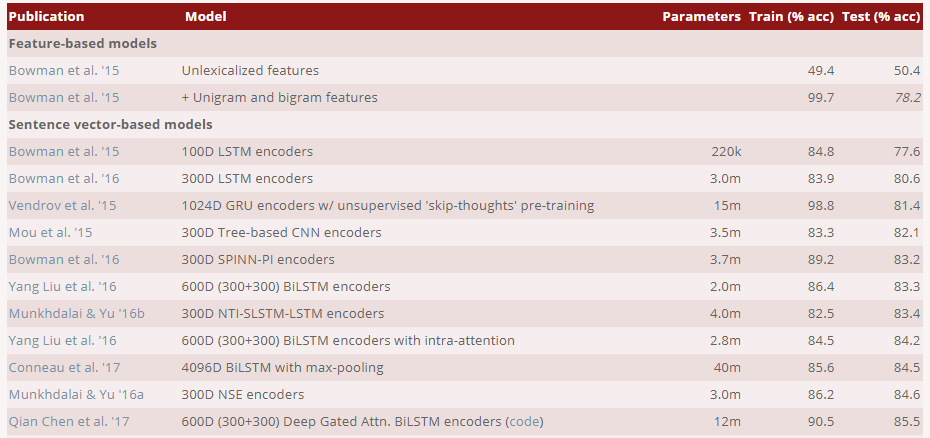
\includegraphics[scale=0.6]{img/snli.png}
                    \caption{A Perspective of Similar Work Performances}
                    \label{fig:snli}
                \end{figure}
                \FloatBarrier
                
                Figure above lists similar work results of recent years, sorted from oldest to newest \autocite{table:snli}. This project falls into the Sentence vector-based models category, so these works are against which the project's performance is going to be compared. As mentioned before, the \gls{lstm} developed here achieves a testing accuracy of 78.13\% which is only slightly above the \textit{100D LSTM encoders} model.
                
                First of all, a bit of context. The numbers with a \textit{D} at the end denote the vector size of the model. These vectors take a lot of \gls{ram} to store them in memory. On top of that, as vector size scales, so do other parameters need to be scaled up, such as the size of \gls{lstm}, for example.
                
                This project uses a vector size of \textit{200D}, which when combined with other \gls{lstm} parameters and the need to store \gls{snli} data in memory for processing, it completely uses up the 16.0 GB of \gls{ram} that the development environment computer has.
                
                When looking at other models that are performing with more accurate results, it is no surprise that they use higher vector sizes, sometimes even multiple vectors or additional components that go hand in hand with \gls{lstm} networks.
                
                In conclusion, it can be said that the model's accuracy is in line with what can and should be expected. On the other hand, it is clear that there is a long way to go to reach super accurate prediction models and even further to be able to run them on home computer conditions for everyday use, such as catching up with social media discussions and online news debates.
            
        \subsubsection{Graph Construction Evaluation} \label{grapheval}
            This section ensures that the functionality of building a graph is working as expected. Among other things, this includes making sure that nodes are created, edges are drawn and differentiated between attack and support and so on.
            
            \begin{figure}[!htbp]
                \centering
                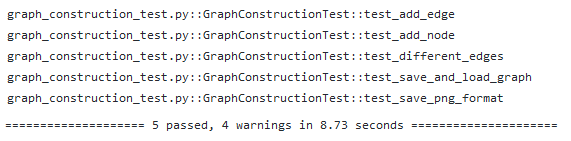
\includegraphics[scale=0.9]{img/graph_construction_test.png}
                \caption{Test Results for Function 4 Requirements}
                \label{fig:testres4}
            \end{figure}
            \FloatBarrier
            
            All of the test cases involve creating a custom graph, which contributed to a higher test running time (8.9 seconds). Requirements 4.1 - 4.3 and 4.7 are tested by simply creating a graph and then assessing if correct nodes, edges or colors are assigned.
            
            For 4.4, 4.5 and 4.8 requirements, the tests are similar in nature to those in \cref{dataeval}. Saved files and their formats are checked by making sure that they exist in the required folder. The loading functionality, however, requires a bit more work to evaluate. First, the graph has to be created and saved, then the graph in memory is set to \textit{null}, or in Python terms, \textit{None}. When the graph is loaded back in, it is evaluated if the same properties remain true that were set during the initial graph creation.
            
            Requirement 4.6 can be tested by simply running the program or any test case that has custom graph in it, can be seen here in \cref{fig:displaygraph} below.
            
            \begin{figure}[!htbp]
                \centering
                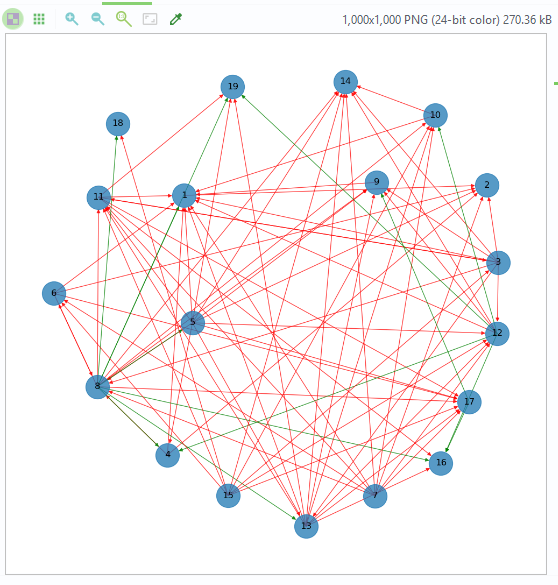
\includegraphics[scale=0.6]{img/display_argument_framework.png}
                \caption{Argument Framework Display}
                \label{fig:displaygraph}
            \end{figure}
            \FloatBarrier
            
            The last requirement, 4.9 is inspected by going into file properties of the image, and checking its' dimensions.
            
            \begin{figure}[!htbp]
                \centering
                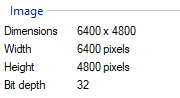
\includegraphics[]{img/high_definition_image_req.png}
                \caption{High Definition Image Dimensions}
                \label{fig:highdef}
            \end{figure}
            \FloatBarrier
            
        \subsubsection{Argument Framework Evaluation} \label{afeval}
            \gls{af} testing requires the creation of a \textit{dummy} \gls{af}, consisting of 4-6 nodes and different relations between them. It is essential to keep the test cases simple and to the point. The requirements 5.1 - 5.3 are tested by assessing the computed conflict free arguments, admissible sets and grounded extension against provided, expected values.
            
            \begin{figure}[!htbp]
                \centering
                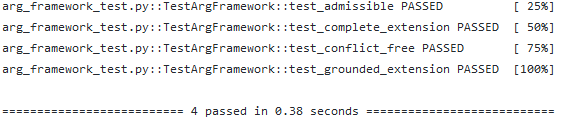
\includegraphics[scale=0.9]{img/arg_framework_test.png}
                \caption{Test Results for Function 5 Requirements}
                \label{fig:testres5}
            \end{figure}
            \FloatBarrier
            
            The remaining requirements, 5.4 - 5.6 are fulfilled as shown in the output log, in \cref{apx_B}.
            
    \subsection{Analysis of Data Mined Argument Frameworks} \label{analysis}
        This section performs an analysis on results generated using this project's software. The main idea here is to analyse what the consensus is with regards to a given topic. The topic will be used as a search term inside Twitter, and the first, most recent tweets will be recorded and argument framework generated out of them.
        
        \subsubsection{Search Term: `Democrats' and `Republicans' Analysis} \label{usaanalysis}
            For this analysis, search terms \textit{Democrats} and \textit{Republicans} were chosen, because those are the two main parties of US government, and intuitively should generate opposing results and view points.
            
            The first argument framework graph is for the search term \textit{Democrats}.
            \begin{figure}[!ht]
                \centering
                \includegraphics[scale=0.3]{img/democrats.png}
                \caption{Argument Framework for `Democrats'}
                \label{fig:demnocrat}
            \end{figure}
            \FloatBarrier
            
            The grounded extension is listed below, including the original, unmodified version of tweets:
            
            \begin{itemize}
                \item Node 7: `@LindseyGrahamSC is absolutely correct  When Democrats talk about needing to ``heal'' the Supreme Court, they mean making it more liberal by any means necessary  It's literal court packing, which should scare every American'
                \item Node 15: `Donald Trump Leads Top Democrats in North Carolina Poll'
                \item Node 18: `@BernieSanders I believe you are describing yourself and other Democrats in Congress who make \$174K per year, yet somehow have accumulated wealth worth \$millions and live in mansions'
            \end{itemize}
            
            Before going any further, same algorithm is run on the term \textit{Republicans}. Here are the results:
            
            \begin{figure}[!htbp]
                \centering
                \includegraphics[scale=0.3]{img/republicans.png}
                \caption{Argument Framework for `Republicans'}
                \label{fig:republican}
            \end{figure}
            \FloatBarrier
            
            And the grounded extension:
            \begin{itemize}
                \item Node 7: `@wiscyfan @TonyBrunoShow @PhillyMayor Most Democrats are corporatists just like Republicans'
                \item Node 8: `@maddow Were the group of Republicans who met w Russians on July 4th from the states Russia asked if interested in investment per your story tonight? Curious, I live in Alabama and Richard Shelby was there'
                \item Node 9: `I’m going to give you a 30 year lesson. Democrats fix the economy, Republicans fuck it up. Stop being fooled by a racist liar. 2020 we have a lot of work to do \#TrumpRecession'
                \item Node 11: `@realNHperson You took the fun out of funny Maybe focus on issues of Republicans rather than latest Democrat obfuscation'
                \item Node 12:` @JohnCornyn Americans don't trust a president that has lied to them over 12,000 times or the Republicans that refuse to hold the corrupt administration accountable because they are profiting off it'
                \item Node 16: `@LindseyGrahamSC When you DON’T HEAR REPUBLICANS SAYING, or DOING ANYTHING to HELP OUR COUNTRY???? but CHOOSE A LYING, CHEATING, THIEF, RAPIST, RACIST, CHILD TRAFFICKER, PEDOPHILIA, ILLITERATE BOY, then WE THE PEOPLE will do EVERYTHING in OUR POWER to MAKE SURE WE DROWN THE COWARDS IN 2020???'
            \end{itemize}
            
            Looking at the graphs, the red arrows represent attacks on arguments and green represent support relations. The large majority of relations are attacks, which is interesting because it implies that due to politics being a controversial subject, people usually express their opinions when they disagree with some points, or are in discontent. On top of that, politics are very subjective in nature, there is not a silver bullet that can solve current political issues, so there might as well be as many opinions as there are people.
            
            The second interesting thing is the fact that when searching for a specific term, the grounded extension is, in this case, a negative opinion involving that query. Neither \textit{democrats} nor \textit{republicans} contain supportive messages in grounded extension, with \textit{republican} \gls{af} not containing a single green arrow.
        
        \subsubsection{Search Term: `Tory' and `Labour' Analysis} \label{ukanalysis}
            The next analysis brings the focus to UK. Here, the terms \textit{Tory} and \textit{Labour} were chosen, which are the two main political parties in UK. With this, the hope is to, first of all, see how these parties are viewed on social media, as they represent the polar opposite ideologies of political spectrum, and secondly, to see if there are any differences or similarities to the previous analysis with the US.
            
            First of all, \gls{af} for the term \textit{Tory}.
            \begin{figure}[!htbp]
                \centering
                \includegraphics[scale=0.3]{img/tory.png}
                \caption{Argument Framework for `Tory'}
                \label{fig:tory}
            \end{figure}
            \FloatBarrier
            
            Accompanied by grounded extension tweets:
            \begin{itemize}
                \item Node 5: `Sarah Wollaston has changed party twice since been elected as a Tory, on a pro-Brexit platform   She once called for MPs switching parties to face automatic by-elections and now refuses to do so herself   Wondering why the public distrust politicians? Sarah is a perfect example'
                \item Node 6: `@LibDems @ChukaUmunna She supported Leave then switched to Remain in last few weeks of EU referendum  Stood on a GE17 Tory Leave manifesto and promised not to back a 2nd referendum  She then backed a 2nd referendum  Sponsored a Bill in HOC for compulsory by-elections for defectors then  defected'
                \item Node 9: `Poverty is no longer a hated symptom, it is a carefully crafted Tory weapon \#dwp \#poverty \#homelessness \#homeless \#OAPs \#PMQs \#pensions \#politics \#parliament \#brexit \#esa \#pips \#wca'
            \end{itemize}
            
            Next, \gls{af} for \textit{Labour}.
            
            \begin{figure}[!htbp]
                \centering
                \includegraphics[scale=0.3]{img/labour.png}
                \caption{Argument Framework for `Labour'}
                \label{fig:labour}
            \end{figure}
            \FloatBarrier
            
            And the grounded extension tweets:
            \begin{itemize}
                \item Node 4: `Jeremy Corbyn has checkmated Jo Swinson \& exposed the Lib Dems again for the vindictive charlatans they are  They've bleated for the last 3 years they want to stop Brexit, they want another vote, but when given the chance by Labour they refuse \#ReachOverTheNoise \#YellowTories'
                \item Node 7: `@GeorgeAylett Ah Labour inflexibility on full show again, combined with its usual effort to blame no deal on everyone else   Nothing to do with the fact that 114 Labour MPs abstained on JC’s orders on the Cherry a Revoke backstop on 1/4/2019    It lost by 112   No deal IS down to LP \& JC''
                \item Node 8: `Sorry, David; I am normally with you on whatever you write   But not with this   You don't seem to understand just how reviled Jeremy Corbyn is!  The man has to be deposed   He has to be got rid of   The Labour Party will only be able to look itself in the mirror afterwards'
                \item Node 14: `@dhothersall No one has yet defined ``brief'' Once in power Labour may move the goalposts - see indyref2 as an example!'
                \item Node 17: `You have been silent for 9 years that @Conservatives have subjected British families to poverty  @UKLabour have tabled a process to block no-deal Brexit while @Conservatives want to shut down Parliament to impose a no-deal  And you still blame Labour, this is perverse'
                \item Node 18: `Agree  and labour are even worse  So we are just country led by Cardiff centric Cartel'
                \item Node 19: `@FaultFinderUK Legal challenge still ongoing (due to Labour's proven use of vote-riggers)  But your bio states that you ``bark at racists'' I suggest you trot on over to Finsbury Park, to the home of your Jew-hating comrade leader currently under investigation for exactly that  There's a good boy'
            \end{itemize}
            
            When comparing the two graphs, it is instantly noticeable that the \gls{af} for \textit{Tory} has quite a few support relations, compared to \textit{Labour}, which has none. A conclusion could be made here that the \textit{Tory} party in the UK, compared to \textit{Labour}, is, at the current political climate, less controversial. Coincidentally, though this is just speculation, it might suggest that people are more in favour of brexit than the news outlets might suggest, because \textit{Tory} party does position itself in favour of leaving the EU.
            
            The \textit{Labour} \gls{af}, on the other hand, not all arguments are specifically against the party. For example, Node 17 from above is clearly arguing for \textit{Labour}. But still, it is undeniable that based on this grounded extension, the opposition party looks to be a lot more controversial.
            
            To contrast this with the US analysis, there are some interesting differences in how the social media treats similar two party government systems. In USA, the discussion involves mainly about the political parties as a whole, with the President's name being mentioned once in a while. UK, on the other hand, has \textit{Party Leaders}. The discussion in UK involves talking about specific actions or stances taken by those individuals who are the faces of the party. It is hard to say why this difference is so stark, but it is interesting nonetheless.

    \subsection{A Review of Project Objectives and Achievements} \label{softachieve}
        This subsection gives an overview of what objectives and aims are achieved at this point. The goal here is to reinforce the reader with concrete examples of accomplishments, specifically with regards to project objectives stated in the beginning. In \cref{aims:objectives}, ten total bullet points were listed, each constituting a project's aim. Here, all bullet points will be referenced to emphasise current achievements.
        
        The first three objectives are to provide an introduction, give technical background on the subject and review existing literature, respectively. \cref{argumentation} and \cref{argumentmining} both give introductions to argumentation as a whole and argument mining. The technical background is extensively covered in \cref{techbackground}, while literature review is presented, critically discussed and evaluated in \cref{literature}. At that point, three aims are already met.
        
        The fourth bullet point states the objective to gather Twitter data, specifically tweets, and preprocess it with the help of stop word elimination and lemmatization. Technical requirements to achieve this are listed in \cref{table:func2spec}, and \cref{twittereval} shows that the requirements are fulfilled. This means that the objective has been met.
        
        Next, the fifth bullet point is concerned with implementing a \gls{lstm} neural network alongside training, validation and testing. Corresponding technical requirements are in \cref{table:func2spec}, and \cref{lstmeval} underlines that proper results are achieved. Another project objective can be crossed off as completed.
        
        The sixth objective tasks the project to recognise textual entailment relationships between tweets. This directly correlates to requirement 3.4 in \cref{table:func3spec}. From \cref{lstmeval} can be seen that this is indeed achieved successfully.
        
        Moving on, the seventh objective says that based on arguments and their relations, a graph representation of it needs to be created. Based on the tests performed in \cref{grapheval} in accordance to \cref{table:func4spec} requirements, it can be noted that a graph was indeed constructed and visually displayed on the screen. This makes the completed objectives count go up to seven out of ten.
        
        The following bullet point is eighth. After the graph representation of \gls{af} is created, the goal is to analyse it and compute the grounded extension, which is exactly what the eighth bullet point states. The previous subsection, namely \cref{afeval}, presents the test results and references technical requirements accordingly (see \cref{table:func5spec} for requirements). The tests indicate that this bullet point has also been met.
        
        The ninth bullet point was done in \cref{usaanalysis} and \cref{ukanalysis} in this chapter. The results were intriguing and gave insight into human behaviour, with, probably, additional analysis possible if performed by a qualified psychologist or anthropology researcher. The latter, the evaluation of neural network and critical comparison of competing models, was done in \cref{similarworkcompare}.
        
        The next two chapters, \cref{conclusions} and \cref{futurework} deal with giving overall conclusions of the project and presenting a discussion of possible future work improvements, respectively. As a matter of fact, this is the last objective from the list, and is fulfilled in the aforementioned sections.